
\documentclass[border=10pt]{standalone}
\usepackage{pgfplots}
\pgfplotsset{compat=1.18}
\begin{document}
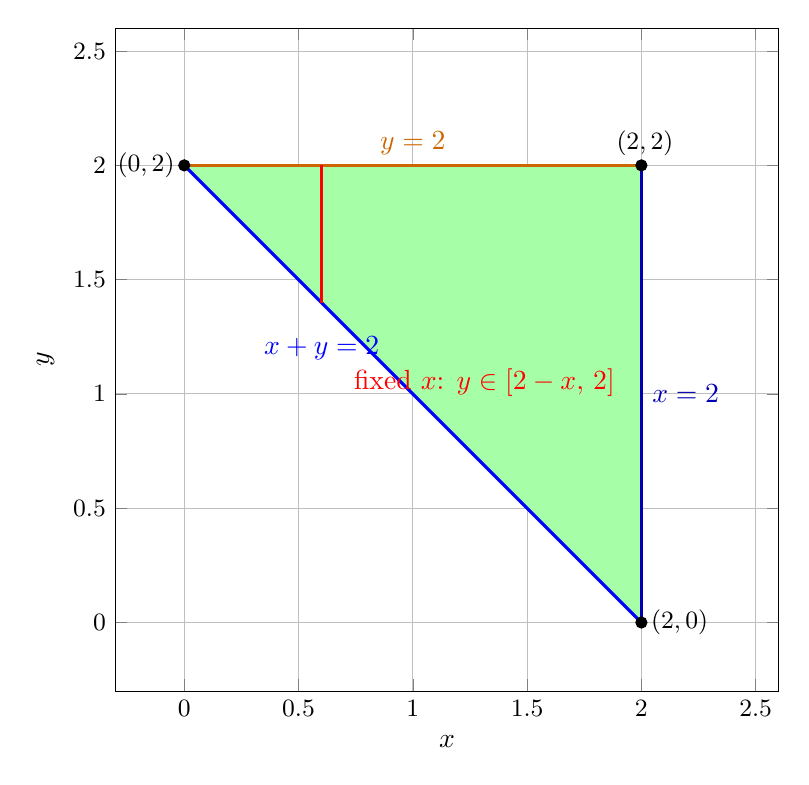
\begin{tikzpicture}
\begin{axis}[
    xlabel={$x$}, ylabel={$y$},
    xmin=-0.3, xmax=2.6, ymin=-0.3, ymax=2.6,
    width=10cm, height=10cm,
    axis equal image,
    grid=both,
    tick label style={font=\small},
]
% filled projection triangle
\addplot[fill=green!35,draw=none] coordinates {(0,2) (2,2) (2,0) (0,2)};
% boundary lines
\addplot[blue,very thick,domain=0:2,samples=2]{2-x} node[pos=0.45,above left]{$x+y=2$};
\addplot[blue!70!black,very thick] coordinates {(2,0) (2,2)} node[pos=0.5,right]{$x=2$};
\addplot[orange!80!black,very thick] coordinates {(0,2) (2,2)} node[pos=0.5,above]{$y=2$};
% fixed-x strip
\addplot[red,very thick] coordinates {(0.6,1.4) (0.6,2)};
\node[red,anchor=west] at (axis cs:0.7,1.05) {fixed $x$: $y\in[2-x,\,2]$};
% vertices
\addplot[only marks,mark=*,mark size=2pt,black] coordinates {(0,2) (2,2) (2,0)};
\node[anchor=east,font=\small] at (axis cs:0,2) {$(0,2)$};
\node[anchor=south,font=\small] at (axis cs:2,2) {\;$(2,2)$};
\node[anchor=west,font=\small] at (axis cs:2,0) {$(2,0)$};
\end{axis}
\end{tikzpicture}
\end{document}
